\documentclass{pfc}

%\usepackage{refcheck} % detectar figures, tablas, etc., no referenciadas

\usepackage{amsmath}
\usepackage{amssymb}
\usepackage{amsfonts}
\usepackage{mathtools}
\usepackage{pdfpages}
\usepackage{subcaption}
\usepackage{gnuplot-lua-tikz}
\usepackage{pstricks}
\usepackage{minted}
\usemintedstyle{bw}
\usepackage{listings}
\lstset{
	literate={~} {$\sim$}{1},
	language=c++,
	basicstyle=\ttfamily,
	keywordstyle=\color{blue},
	commentstyle=\color{dkgreen},
	stringstyle=\color{red},
	breaklines=true,
	breakatwhitespace=true,
	tabsize=4
}

\usepackage[noabbrev]{cleveref}

\subtitle{Informe final}

\newcommand{\TODO}[1]{{\color{red}\bfseries#1}}
\newcommand{\Nota}[1]{{\color{blue}\itshape#1}}

\newcommand{\CasoUso}[1]{\bigskip%
{\bfseries Caso de uso: #1}\par}
\newcommand{\IncCU}[1]{{\bfseries Include (#1)}}
\newcommand{\UseCU}[1]{{\bfseries Use (#1)}}
\newcommand{\CUField}[2]{{\bfseries#1:} #2\par}
\newcommand{\CUNormal}{{\bfseries Curso Normal:}\par}

\newenvironment{CasoDeUso}[1]{%
	\bigskip\begin{minipage}{.9\linewidth}
		{\bfseries Caso de uso: #1}\par
}
{%
	\end{minipage}
}


\newcommand{\Requerimiento}[2]{%
	\bigskip%
	{\bfseries #1}\\%
	#2%
}

\usepackage{algorithmicx}
\usepackage{algorithm}
\usepackage[noend]{algpseudocode}
\usepackage{booktabs}


\makeatletter
 \renewcommand{\ALG@name}{Algoritmo}
\makeatother
\renewcommand{\algorithmicfunction}{}

%\newcommand{\Alerta}[1]{{\Huge\bfseries\sffamily#1}}
\newcommand{\NombreItem}[1]{{\bfseries#1:}}

\usepackage{tikz}
\usetikzlibrary{arrows,chains,matrix,positioning,scopes}

\usepackage{environ}
\makeatletter
\newsavebox{\measure@tikzpicture}
\NewEnviron{scaletikzpicturetowidth}[1]{%
  \def\tikz@width{#1}%
  \def\tikzscale{1}\begin{lrbox}{\measure@tikzpicture}%
  \BODY
  \end{lrbox}%
  \pgfmathparse{#1/\wd\measure@tikzpicture}%
  \edef\tikzscale{\pgfmathresult}%
  \BODY
}
\makeatother

\newcommand{\bigO}{\mathcal{O}}
\newcommand{\Real}{\mathbb{R}}
\DeclareMathOperator*{\argmin}{argmin}
\DeclareMathOperator{\atan}{atan}

\graphicspath{{./uml/}{./diagram/}{./graph/}}

\newcommand{\RefImagen}[1]{ (Imagen cortesía de \cite{#1})}

\newcommand{\Em}{\hspace{1em}}

%\includeonly{reconstrucción}
\begin{document}
\frontmatter
%\TODO{revisar tiempos verbales, ahora en pasado}
	\maketitle

	\chapter{Resumen}
Gracias a los avances en sensores de profundidad y técnicas de reconstrucción de superficies,
es posible obtener con gran precisión una nube de puntos que represente
la forma, posición y dimensiones de un objeto cualquiera.
Sin embargo, esta nube de puntos es parcial, ya que solamente refleja
la porción observable desde el punto de captura.
Por esta razón, en este proyecto se propone el desarrollo de una biblioteca de software
que implemente técnicas para combinar estas vistas parciales
y así obtener un modelo tridimensional de todo el objeto,
posibilitando su posterior construcción mediante técnicas de impresión 3D.

\Nota{
	sensores de profundidad y técnicas para determinar la profundidad.

	Hablar de prime-sense, kinect fusion, que requieren que el usuario
	tome las capturas con mucho cuidado

	Nosotros hacemos pocas capturas espaciadas, esa es la gracia
%TODO: motivación continuar lo de pancho
%explayarse en la forma de adquisición
%vistas parciales
}
	%\noindent{\bfseries Palabras clave:} fusión de mallas, imágenes de profundidad, impresión 3D, reconstrucción 3D.


	\tableofcontents
	\listoffigures

\mainmatter
	\include{introduccion}
	\include{reconstruccion}
	\section{Base de datos}
Uno de los supuestos de este proyecto era contar con un repositorio propio de
mallas tridimensionales.
Para la creación de este repositorio,
se utilizarían los algoritmos de reconstrucción desarrollados en \cite{Pancho},
ubicando al objeto de interés end una base giratoria y realizando capturas
en ángulos espaciados hasta completar una vuelta.
De esta forma, las posiciones de las vistas describirían un círculo centrado en el objeto y
cada captura contendría información de posición ($xyz$) y de textura ($rgb$).
Debido a los tiempos requeridos para calibrar el dispositivo de captura,
este repositorio nunca se materializó,
 por lo que fue necesario buscar otro con características similares.

%\begin{itemize}
%	\item redwood, freibug:
%	rgb y profundidad, pero el movimiento es pequeño y libre
%	(tendría que eliminar intermedios)
%\item middlebury
%	base giratoria, pero sólo RGB
%	(tendría que generar el mapa de profundidad)
%\item stanford
%	base giratoria, nube de puntos, sin textura.
%	Se optó por esta.
%	Se decidió no generar artificialmente los puntos de textura para tener un
%	caso más real.
%\end{itemize}

Se decidió utilizar \emph{The Stanford 3D Scanning Repository}\cite{StanfordScanRep} que brinda
acceso a escaneos tridimensionales y reconstrucciones detalladas para ser
usados en investigación.

Las capturas fueron obtenidas mediante un escáner láser de barrido Cyberware
3030~MS.  Se realizaron escaneos del objeto en diversas posiciones sobre una
base giratoria y luego estas capturas fueron combinadas para producir una única
malla triangular utilizando el método de \emph{zippering} o el de
\emph{volumetric merging}, ambos desarrollados en
Stanford\cite{StanfordScanRep}. \Nota{si no explico esos métodos, volarlos de acá\\}

La base de datos provee un archivo de configuración con las transformaciones de
alineación requeridas por cada captura.
Estas transformaciones fueron obtenidas realizando la registración de cada captura
contra un escaneo cilíndrico del objeto mediante un método semiautomático, donde el usuario
usuario establece una alineación inicial que luego es ajustada mediante un algoritmo
basado en ICP\cite{Turk:1994:ZPM:192161.192241}.

De esta base de datos se utilizaron los modelos
	\texttt{armadillo},
	\texttt{bunny},
	\texttt{dragon},
	\texttt{drill} y
	\texttt{happy},
los cuales presentan distintos niveles de detalles, cantidad de escaneos y niveles de ruido.


\begin{figure}
	\Imagen{example-image-a}
	\caption{\label{fig:stanfod_models}\TODO{Modelos de la base de datos Stanford.}}
\end{figure}


Desgraciadamente, no se cuenta con información de color en estos escaneos.
Se decidió adaptar los algoritmos a esta situación, en lugar de agregar
artificialmente valores de color para los puntos.


\section{Tecnologías}
	%Intro
	A continuación se mencionan las principales herramientas de software
	utilizadas en el desarrollo de programas de reconstrucción tridimensional.

	\subsection{KinectFusion}
	Es el algoritmo desarrollado por Microsoft para lograr reconstrucciones
	tridimensionales utilizando el dispositivo Kinect.

	%kinectfusion_real-time_3d_reconstruction_and_interaction_using_a_moving_depth_camera
	Debido a que uno de sus objetivos era lograr una implementación en tiempo
	real, el algoritmo de registración requiere de poca variación
	de la posición relativa cámara-objeto entre capturas, por lo que no fue utilizado.

	Para realizar la fusión utiliza una variación del método de
	\emph{volumetric merging} sobre GPU.\cite{Izadi:2011:KRR:2047196.2047270}

	%Suposiciones:
	%transforma el sistem en uno lineal, la transformación entre capturas es un incremento pequeño
	%sistema 6x6 (3 translaciones, 3 rotaciones)
	%utiliza todos los puntos porque tiene gpu




	\subsection{Open Source Computer Vision Library (OpenCV)}
	Es una biblioteca de código abierto de visión computacional y aprendizaje
	maquinal.  Cuenta con módulos de procesamiento de imágenes de profundidad y
	registración.

	En un principio se consideró utilizar la información de textura de las
	capturas para poder lograr la registración, pero debido a que la base de
	datos utilizada sólo contenía información geométrica  no se utilizarán las
	funcionalidades de esta biblioteca.

	\subsection{\emph{The Point Cloud Library} (PCL)}
	Es un framework de código abierto multiplataforma para el procesado de
	imágenes 2D/3D y nubes de puntos.
	Provee numerosos algoritmos modernos para reducción de ruido, extracción de
	puntos salientes, cálculo de descriptores, registración, reconstrucción de
	superficies, entre otros.

	La documentación incluye tutoriales para cada módulo de la biblioteca y
	además se cuenta con listas de correos y canales de IRC para brindar
	soporte.

	PCL se encuentra disponible para ser usada en C++.
	Debido al uso intensivo de código templatizado, la compilación del
	código cliente requiere de un tiempo considerable (aproximadamente un minuto).
	Existen proyectos para portarla a Python y Java, pero no se encuentran
	suficientemente avanzados.

	\subsection{CloudCompare, Meshlab}
	Son programas de procesamiento y edición de mallas de puntos 3D.  Presentan
	herramientas de registración semiautomática (a partir de puntos
	seleccionados por el usuario), y cuentan con una implementación del
	algoritmo \emph{Poisson Surface Reconstruction} para reconstrucción de
	superficies.

	Se utilizarán especialmente para visualización y comparación de resultados.



	\include{diseno}
	\documentclass{pfc}
\title{Casos de uso}
\author{Walter Bedrij}
\date{\today}

\begin{document}
	\CasoUso{Ingresar lista de mallas}
		\Actor{Programador}
	\CasoUso{Ajustar parámetros}
		\Actor{Programador}
	\CasoUso{Alinear dos mallas}
		\Actor{Programador}
	\CasoUso{Corregir error de bucle}
		\Actor{Programador}
	\CasoUso{Rechazar malla}
		\Actor{Programador}
	\CasoUso{Extraer superficie}
		\Actor{Programador}
	\CasoUso{Rellenar huecos}
		\Actor{Programador}
\end{document}

\section{Especificación de requerimientos}
A partir del análisis de las herramientas de software existentes,
el estudio de la bibliografía relevante y el diagrama de los casos de uso
se definió el siguiente documento de requerimientos

\subsection{Descripción}
	Se dispone de un sistema cámara-superficie giratoria, cuyas posiciones
	se encuentran fijas en el espacio y el eje de giro de la superficie se
	encuentra alineado con el eje vertical del dispositivo de captura.
	El objeto de interés se ubica sobre la superficie giratoria, y se
	realizan capturas a diversos intervalos de giro
	hasta totalizar una vuelta completa (360\textdegree).

	Los algoritmos desarrollados para la registración de las capturas parciales,
	integración de las mallas resultantes y rellenado de huecos tendrán como resultado final
	una superficie cerrada triangulada que represente al objeto.

	Se tendrá como entrada una nube de puntos con valores de posición $\{x, y, z\}$.
	No se dispondrá de información de textura, normales o conectividades.

	\subsubsection{Suposiciones}
		El ángulo máximo entre dos mallas no podrá exceder los 60\textdegree.

		La cámara no se encontrará demasiado elevada respecto a la
		superficie giratoria. En ningún caso deberá superar el punto más alto del objeto.

\subsection{Requerimientos funcionales}
Se identificaron las siguientes funcionalidades para el sistema:

	\Requerimiento
		{Eliminación de puntos atípicos}
		{El sistema debe detectar y eliminar puntos considerados atípicos.}

	\Requerimiento
		{Alineación Inicial}
		{El sistema debe poder calcular una transformación de alineación para dos mallas
		que las acerque lo suficiente como para poder utilizar luego ICP.}

	\Requerimiento
		{Área solapada}
		{El sistema debe poder establecer los puntos en común (o una buena
		aproximación) entre dos mallas ya alineadas burdamente.}

	\Requerimiento
		{Métricas}
		{El sistema debe poder evaluar la calidad de una registración.}

	\Requerimiento
		{Corrección de bucle}
		{El sistema debe corregir el error propagado durante la registración
		una vez que se haya realizado una vuelta con las capturas.}

	\Requerimiento
		{Combinación de nubes}
		{El sistema debe generar una malla de consenso, ajustando los puntos y sus normales
		según la información provista por cada malla de entrada.}

	\Requerimiento
		{Triangulación}
		{El sistema debe poder triangular una nube de puntos tridimensional.}

	\Requerimiento
		{Relleno}
		{El sistema debe disponer de funciones para lograr que una malla sea cerrada. Se
		estimará una superficie en las zonas donde se carezca de
		información.}

\subsection{Requerimientos no funcionales}
	Se identificaron los siguientes requerimientos no funcionales:

	\Requerimiento{Tiempo de ejecución}
	{No se espera una ejecución a tiempo real de los algoritmos implementados.}

	\Requerimiento{Interfaces con software}
	{Las operaciones sobre las mallas y nubes de puntos se realizará
	mediante la \emph{Point Cloud Library} (PCL).
	Debido a esto, se desarrollará en el lenguaje de programación C++.}


	\Requerimiento{Sistemas operativos}
	{El producto desarrollado estará destinado a utilizarse en los sistemas
	operativos Windows y Linux.}

\chapter{Diseño}
En este capítulo se presentarán los requerimientos identificados para el sistema
y los diagramas de clases definidos para su implementación.

\documentclass{pfc}
\title{Casos de uso}
\author{Walter Bedrij}
\date{\today}

\begin{document}
	\CasoUso{Ingresar lista de mallas}
		\Actor{Programador}
	\CasoUso{Ajustar parámetros}
		\Actor{Programador}
	\CasoUso{Alinear dos mallas}
		\Actor{Programador}
	\CasoUso{Corregir error de bucle}
		\Actor{Programador}
	\CasoUso{Rechazar malla}
		\Actor{Programador}
	\CasoUso{Extraer superficie}
		\Actor{Programador}
	\CasoUso{Rellenar huecos}
		\Actor{Programador}
\end{document}

\section{Especificación de requerimientos}
A partir del análisis de las herramientas de software existentes,
el estudio de la bibliografía relevante y el diagrama de los casos de uso
se definió el siguiente documento de requerimientos

\subsection{Descripción}
	Se dispone de un sistema cámara-superficie giratoria, cuyas posiciones
	se encuentran fijas en el espacio y el eje de giro de la superficie se
	encuentra alineado con el eje vertical del dispositivo de captura.
	El objeto de interés se ubica sobre la superficie giratoria, y se
	realizan capturas a diversos intervalos de giro
	hasta totalizar una vuelta completa (360\textdegree).

	Los algoritmos desarrollados para la registración de las capturas parciales,
	integración de las mallas resultantes y rellenado de huecos tendrán como resultado final
	una superficie cerrada triangulada que represente al objeto.

	Se tendrá como entrada una nube de puntos con valores de posición $\{x, y, z\}$.
	No se dispondrá de información de textura, normales o conectividades.

	\subsubsection{Suposiciones}
		El ángulo máximo entre dos mallas no podrá exceder los 60\textdegree.

		La cámara no se encontrará demasiado elevada respecto a la
		superficie giratoria. En ningún caso deberá superar el punto más alto del objeto.

\subsection{Requerimientos funcionales}
Se identificaron las siguientes funcionalidades para el sistema:

	\Requerimiento
		{Eliminación de puntos atípicos}
		{El sistema debe detectar y eliminar puntos considerados atípicos.}

	\Requerimiento
		{Alineación Inicial}
		{El sistema debe poder calcular una transformación de alineación para dos mallas
		que las acerque lo suficiente como para poder utilizar luego ICP.}

	\Requerimiento
		{Área solapada}
		{El sistema debe poder establecer los puntos en común (o una buena
		aproximación) entre dos mallas ya alineadas burdamente.}

	\Requerimiento
		{Métricas}
		{El sistema debe poder evaluar la calidad de una registración.}

	\Requerimiento
		{Corrección de bucle}
		{El sistema debe corregir el error propagado durante la registración
		una vez que se haya realizado una vuelta con las capturas.}

	\Requerimiento
		{Combinación de nubes}
		{El sistema debe generar una malla de consenso, ajustando los puntos y sus normales
		según la información provista por cada malla de entrada.}

	\Requerimiento
		{Triangulación}
		{El sistema debe poder triangular una nube de puntos tridimensional.}

	\Requerimiento
		{Relleno}
		{El sistema debe disponer de funciones para lograr que una malla sea cerrada. Se
		estimará una superficie en las zonas donde se carezca de
		información.}

\subsection{Requerimientos no funcionales}
	Se identificaron los siguientes requerimientos no funcionales:

	\Requerimiento{Tiempo de ejecución}
	{No se espera una ejecución a tiempo real de los algoritmos implementados.}

	\Requerimiento{Interfaces con software}
	{Las operaciones sobre las mallas y nubes de puntos se realizará
	mediante la \emph{Point Cloud Library} (PCL).
	Debido a esto, se desarrollará en el lenguaje de programación C++.}


	\Requerimiento{Sistemas operativos}
	{El producto desarrollado estará destinado a utilizarse en los sistemas
	operativos Windows y Linux.}

%diagramas de clases

\input{pruebas}


	\chapter{Pruebas y resultados}
	A continuación se detallan las pruebas realizadas y los resultados obtenidos
	por cada módulo desarrollado utilizando como base los modelos
	\texttt{armadillo}, \texttt{bunny}, \texttt{dragon}, \texttt{drill} y \texttt{happy}
	del repositorio de Stanford\cite{StanfordScanRep}.

	\section{Módulo de registración}
	Para la registración se utilizó el método basado en la búsqueda de clúster,
	seguido de un refinamiento mediante ICP y una corrección de bucle.
	Se plantearon dos métodos para evaluar la calidad de cada registración:
	\begin{itemize}
		\item Mediante la comparación entre la transformación calculada y aquella provista por la base de datos (\emph{ground truth}).
		\item Mediante una métrica de \emph{fitness} que se obtiene a partir de la nube transformada y las nubes de entrada.
	\end{itemize}

	Para comparar las alineaciones contra el \emph{ground truth}, se
	observa el efecto de las mismas sobre un punto orientado simulando la
	cámara (figura~\ref{fig:err_reg}). El punto \emph{eye} ($C$) se ubica inicialmente en las coordenadas
	$\{0, -0.1, 0.7\}$ (valores obtenidos de la base de datos), y se
	orienta el vector \emph{target} hacia $-z$ y el \emph{up} hacia $y$.
	El error de posicionamiento es la razón entre la distancia al punto
	de inicio y la distancia al punto obtenido por el \emph{ground truth}.
	\[\text{Error} = \frac{|C'-C_{gt}|}{|C_{gt} - C|}\]
	Los errores de \emph{target} y \emph{up} se corresponden al ángulo formado contra los
	vectores respectivos obtenidos por el \emph{ground truth}.

	\begin{figure}
		\centering
		\input{diagram/error_registration.pdf_tex}
		\caption{\label{fig:err_reg}Comparación entre las transformaciones de alineación.
		Se observa el efecto producido en un punto orientado $C$ que simula la posición de la cámara.}
	\end{figure}

	En el cuadro~\ref{tab:reg_error} se presentan los errores de registración promedio para cada orientación de los modelos.
	En la mayoría de los casos, los errores no superan $1^{\circ}$ en orientación ni $1\%$ en posicionamiento,
	observándose dos excepciones: \texttt{bunny} y \texttt{dragon stand}.
	El aumento en el error del modelo \texttt{bunny} se debe a que la captura \texttt{bun180} presenta una distancia cercana a $90^\circ$,
	superando las restricciones impuestas en este trabajo.
	Sin embargo, en el caso de \texttt{dragon stand} el error refleja una mala
	alineación en la captura~12, debida a una mala selección de los parámetros.
	Mediante un posterior ajuste de los parámetros, en particular, del tamaño de la vecindad para el cálculo de los descriptores, se obtuvo una alineación correcta.

	\begin{table}
	\centering
	\begin{tabular}{l*{3}{c}}
		\toprule
		Modelo                   &    Eye          &    Target (grados)        &    Up (grados)\\
		\midrule
		armadillo\\
		{\Em}back          &     0.0062159   &   0.221725     &    0.15211\\
		{\Em}head          &     0.0036356  &    0.102321     &    0.211231\\
		{\Em}head offset   &     0.0029806  &    0.086309     &    0.229574\\
		{\Em}stand         &     0.0022145  &    0.049612     &    0.105862\\
		{\Em}stand flip    &     0.0045019  &    0.125330     &    0.146033\\
		\midrule
		bunny                   &     0.0104809   &   0.598354     &    0.817185\\
		\midrule
		dragon\\
		{\Em}side             &     0.0070872  &    0.178650     &    0.212932\\
		{\Em}stand            &     0.0536199   &   1.379760     &    0.207754\\
		{\Em}up               &     0.0058265  &    0.139297     &    0.0675651\\
		\midrule
		drill                   &     0.0082317  &    0.238639     &    0.100126\\
		\midrule
		happy\\
		{\Em}back              &     0.0088540  &    0.189885     &    0.207247\\
		{\Em}side              &     0.0072675   &   0.175860     &    0.17525\\
		{\Em}stand             &     0.0050124  &    0.101383     &    0.097800\\
		\bottomrule
	\end{tabular}
	\caption[Errores de registración]{\label{tab:reg_error}Errores de registración.}
\end{table}


	Para evaluar la alineación entre un par de capturas prescindiendo del \emph{ground truth}, y situándonos en un escenario más realista,
	se diseñó una medida de \emph{fitness}.
	Esta medida se define como el porcentaje del área solapada entre las nubes una vez alineadas,
	donde un bajo solapamiento nos indicaría un posible error de alineación, como
	se observa en la figura~\ref{fig:fitness}.

	\TODO{explicar que el cambio de la vecindad lo resuelve}

	\begin{figure}
		\centering
			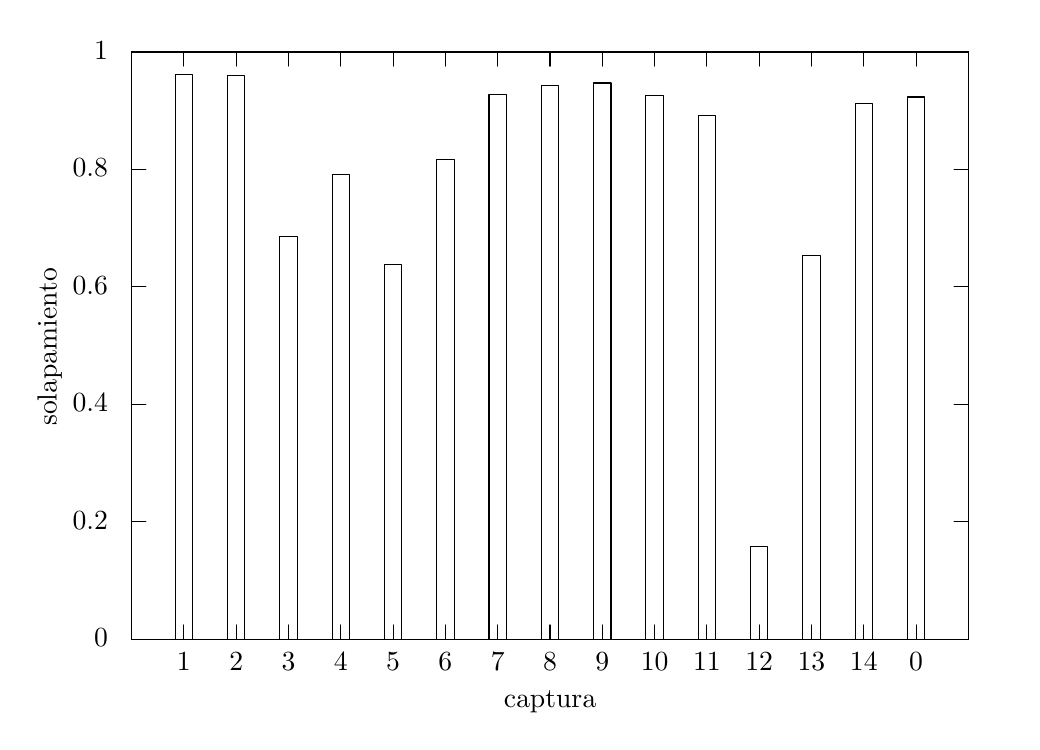
\begin{tikzpicture}[gnuplot]
%% generated with GNUPLOT 5.4p0 (Lua 5.4; terminal rev. Jun 2020, script rev. 114)
%% Tue 25 Aug 2020 01:55:34 AM -03
\gpmonochromelines
\path (0.000,0.000) rectangle (12.500,8.750);
\gpcolor{color=gp lt color border}
\gpsetlinetype{gp lt border}
\gpsetdashtype{gp dt solid}
\gpsetlinewidth{1.00}
\draw[gp path] (1.320,0.985)--(1.500,0.985);
\draw[gp path] (11.947,0.985)--(11.767,0.985);
\node[gp node right] at (1.136,0.985) {$0$};
\draw[gp path] (1.320,2.476)--(1.500,2.476);
\draw[gp path] (11.947,2.476)--(11.767,2.476);
\node[gp node right] at (1.136,2.476) {$0.2$};
\draw[gp path] (1.320,3.967)--(1.500,3.967);
\draw[gp path] (11.947,3.967)--(11.767,3.967);
\node[gp node right] at (1.136,3.967) {$0.4$};
\draw[gp path] (1.320,5.459)--(1.500,5.459);
\draw[gp path] (11.947,5.459)--(11.767,5.459);
\node[gp node right] at (1.136,5.459) {$0.6$};
\draw[gp path] (1.320,6.950)--(1.500,6.950);
\draw[gp path] (11.947,6.950)--(11.767,6.950);
\node[gp node right] at (1.136,6.950) {$0.8$};
\draw[gp path] (1.320,8.441)--(1.500,8.441);
\draw[gp path] (11.947,8.441)--(11.767,8.441);
\node[gp node right] at (1.136,8.441) {$1$};
\draw[gp path] (1.984,0.985)--(1.984,1.165);
\draw[gp path] (1.984,8.441)--(1.984,8.261);
\node[gp node center] at (1.984,0.677) {1};
\draw[gp path] (2.648,0.985)--(2.648,1.165);
\draw[gp path] (2.648,8.441)--(2.648,8.261);
\node[gp node center] at (2.648,0.677) {2};
\draw[gp path] (3.313,0.985)--(3.313,1.165);
\draw[gp path] (3.313,8.441)--(3.313,8.261);
\node[gp node center] at (3.313,0.677) {3};
\draw[gp path] (3.977,0.985)--(3.977,1.165);
\draw[gp path] (3.977,8.441)--(3.977,8.261);
\node[gp node center] at (3.977,0.677) {4};
\draw[gp path] (4.641,0.985)--(4.641,1.165);
\draw[gp path] (4.641,8.441)--(4.641,8.261);
\node[gp node center] at (4.641,0.677) {5};
\draw[gp path] (5.305,0.985)--(5.305,1.165);
\draw[gp path] (5.305,8.441)--(5.305,8.261);
\node[gp node center] at (5.305,0.677) {6};
\draw[gp path] (5.969,0.985)--(5.969,1.165);
\draw[gp path] (5.969,8.441)--(5.969,8.261);
\node[gp node center] at (5.969,0.677) {7};
\draw[gp path] (6.634,0.985)--(6.634,1.165);
\draw[gp path] (6.634,8.441)--(6.634,8.261);
\node[gp node center] at (6.634,0.677) {8};
\draw[gp path] (7.298,0.985)--(7.298,1.165);
\draw[gp path] (7.298,8.441)--(7.298,8.261);
\node[gp node center] at (7.298,0.677) {9};
\draw[gp path] (7.962,0.985)--(7.962,1.165);
\draw[gp path] (7.962,8.441)--(7.962,8.261);
\node[gp node center] at (7.962,0.677) {10};
\draw[gp path] (8.626,0.985)--(8.626,1.165);
\draw[gp path] (8.626,8.441)--(8.626,8.261);
\node[gp node center] at (8.626,0.677) {11};
\draw[gp path] (9.290,0.985)--(9.290,1.165);
\draw[gp path] (9.290,8.441)--(9.290,8.261);
\node[gp node center] at (9.290,0.677) {12};
\draw[gp path] (9.954,0.985)--(9.954,1.165);
\draw[gp path] (9.954,8.441)--(9.954,8.261);
\node[gp node center] at (9.954,0.677) {13};
\draw[gp path] (10.619,0.985)--(10.619,1.165);
\draw[gp path] (10.619,8.441)--(10.619,8.261);
\node[gp node center] at (10.619,0.677) {14};
\draw[gp path] (11.283,0.985)--(11.283,1.165);
\draw[gp path] (11.283,8.441)--(11.283,8.261);
\node[gp node center] at (11.283,0.677) {0};
\draw[gp path] (1.320,8.441)--(1.320,0.985)--(11.947,0.985)--(11.947,8.441)--cycle;
\node[gp node center,rotate=-270] at (0.292,4.713) {solapamiento};
\node[gp node center] at (6.633,0.215) {captura};
\draw[gp path] (1.873,0.985)--(1.873,8.158)--(2.095,8.158)--(2.095,0.985)--cycle;
\draw[gp path] (2.538,0.985)--(2.538,8.144)--(2.759,8.144)--(2.759,0.985)--cycle;
\draw[gp path] (3.202,0.985)--(3.202,6.102)--(3.423,6.102)--(3.423,0.985)--cycle;
\draw[gp path] (3.866,0.985)--(3.866,6.882)--(4.087,6.882)--(4.087,0.985)--cycle;
\draw[gp path] (4.530,0.985)--(4.530,5.745)--(4.752,5.745)--(4.752,0.985)--cycle;
\draw[gp path] (5.194,0.985)--(5.194,7.078)--(5.416,7.078)--(5.416,0.985)--cycle;
\draw[gp path] (5.859,0.985)--(5.859,7.902)--(6.080,7.902)--(6.080,0.985)--cycle;
\draw[gp path] (6.523,0.985)--(6.523,8.015)--(6.744,8.015)--(6.744,0.985)--cycle;
\draw[gp path] (7.187,0.985)--(7.187,8.047)--(7.408,8.047)--(7.408,0.985)--cycle;
\draw[gp path] (7.851,0.985)--(7.851,7.892)--(8.073,7.892)--(8.073,0.985)--cycle;
\draw[gp path] (8.515,0.985)--(8.515,7.634)--(8.737,7.634)--(8.737,0.985)--cycle;
\draw[gp path] (9.180,0.985)--(9.180,2.163)--(9.401,2.163)--(9.401,0.985)--cycle;
\draw[gp path] (9.844,0.985)--(9.844,5.858)--(10.065,5.858)--(10.065,0.985)--cycle;
\draw[gp path] (10.508,0.985)--(10.508,7.788)--(10.729,7.788)--(10.729,0.985)--cycle;
\draw[gp path] (11.172,0.985)--(11.172,7.869)--(11.394,7.869)--(11.394,0.985)--cycle;
\draw[gp path] (1.320,8.441)--(1.320,0.985)--(11.947,0.985)--(11.947,8.441)--cycle;
%% coordinates of the plot area
\gpdefrectangularnode{gp plot 1}{\pgfpoint{1.320cm}{0.985cm}}{\pgfpoint{11.947cm}{8.441cm}}
\end{tikzpicture}
%% gnuplot variables

		\caption[Métrica de alineación para el modelo \texttt{dragon stand}]{\label{fig:fitness}Métrica de alineación para el modelo \texttt{dragon stand}. El bajo
		porcentaje de solapamiento en la captura 12 se corresponde
		con un error de registración.}
	\end{figure}


	\section{Módulo de fusión}
	%En la fusión se utilizó una distancia de proximidad de $1.5$ veces la resolución de las nubes,
	%y un mínimo de confianza de $0.2$.

	Como medida de error de la fusión se utilizó la distancia entre los puntos de la nube reconstruida
	respecto al punto más cercano en el \emph{ground truth} (cuadro~\ref{tab:fus_error}).
	Esta medición no se realizó para el modelo \texttt{armadillo} debido a que su reconstrucción
	se encontraba a una escala distinta a la de las capturas.
	Nuevamente se destaca el error de \texttt{dragon stand} producto de una mala alineación.

	\begin{table}
	\center
	\begin{tabular}{l*{3}{c}}
		\toprule                                                                  
		Modelo                  &    Error promedio  & Desvío \\ 
		\midrule                                    
		bunny                   &      1.28464       & 0.74131\\
		\midrule                                    
		dragon side             &      1.19651       & 0.69846\\
		dragon stand            &      2.83930       & 2.41398\\
		dragon up               &      1.14363       & 0.88966\\
		\midrule                                    
		drill (contra vrip)     &      1.48515       & 0.96336\\
		drill (contra zip)      &      1.74326       & 1.39883\\
		\midrule                                    
		happy back              &      1.65632       & 1.27056\\
		happy side              &      1.35371       & 1.01163\\
		happy stand             &      1.79513       & 1.25758\\
		\bottomrule                                                               
	\end{tabular}
	\caption{\label{tab:fus_error}Errores en la fusión, normalizados respecto a la resolución de las capturas.}
\end{table}



	En todos los modelos, se observa, además, una inflación/deflación de los objetos
	reconstruidos debida a la propagación del error de alineación.  Así, la
	primera captura coincide casi exactamente, pero el error se incrementa
	a medida que nos alejamos de ella (figura~\ref{fig:fus_happy}).

	\begin{figure}
		\Imagen{img/happy_diff}
		\caption[Medida de error en la fusión]{\label{fig:fus_happy}Diferencia contra el \emph{ground truth} del modelo \texttt{happy}.}
	\end{figure}

	\section{Módulo de rellenado de huecos}
		\subsection{Método de advancing front}
		Al utilizar el método de advancing front sobre la superficie reconstruida de \texttt{bunny},
		se logró el rellenado de agujeros pequeños, obteniéndose una malla regular (figura~\ref{fig:fill_good}).
		Sin embargo, debido a la localidad con la que se generan los nuevos
		puntos, el frente puede diverger o pretender unirse a puntos que no
		forman parte del contorno del hueco, resultando una malla mal formada,
		con aristas que corresponden a más de dos caras (figura~\ref{fig:fill_bad}).
		Por estas razones, el método no resulta adecuado para el rellenado automático.


		\begin{figure}
			\Imagen{img/fill_good}
			\caption[Relleno de un hueco pequeño mediante \emph{advancing front}]
			{\label{fig:fill_good}Relleno de un hueco pequeño mediante \emph{advancing front}.}
		\end{figure}

		\begin{figure}
			\Imagen{img/fill_bad}
			\caption[Fallo en el algoritmo de \emph{advancing front}]
			{\label{fig:fill_bad}Fallo en el algoritmo de \emph{advancing front}.
			Se intentó completar un triángulo con un punto que no pertenecía al borde.}
		\end{figure}

		\subsection{Reconstrucción de Poisson}
		Como se mencionó anteriormente, la reconstrucción de Poisson nos garantiza el
		rellenado de todos los huecos (a excepción de la base) mediante una superficie suave.
		Se procedió, entonces, a una valoración visual de los objetos reconstruidos (figura~\ref{fig:poiss_all}):
		\begin{itemize}
			\item En \texttt{bunny} (figura~\ref{fig:bun_ear}) se observan desperfectos debidos a una mala registración de la captura \texttt{bun180},
				que se encontraba aproximadamente a $90^{\circ}$ respecto a sus vecinos.
			\item En \texttt{drill} (figura~\ref{fig:drill_drops}) se tienen componentes inconexas debido a una mala fusión en una zona de alta curvatura.
			\item En \texttt{dragon}(figura~\ref{fig:dragon_belly}) se observa la creación de un puente entre dos regiones.
				Esta es una de las limitaciones conocidas del método, al no poder incorporar la información de línea de vista de las capturas\cite{Kazhdan:2006:PSR:1281957.1281965}.
			\item En todos los casos, la base de apoyo del objeto presenta una deformación hacia abajo (figura~\ref{fig:base}) con un hueco al final.
		\end{itemize}

		\begin{figure}
			\Imagen{img/models_b}
			\caption[Resultado de las reconstrucciones]{\label{fig:poiss_all}Resultado de las reconstrucciones luego del rellenado de huecos mediante el método de Poisson.
			De izquierda a derecha y de arriba a abajo, los modelos son:
			\texttt{armadillo},
			\texttt{bunny},
			\texttt{dragon},
			\texttt{drill}
			y \texttt{happy}.}
		\end{figure}

		\begin{figure}
			\centering
			\includegraphics[max width=.5\linewidth, max height=.25\textheight, keepaspectratio]
				{img/bunny_ear}
			%\Imagen{img/bunny_ear}
			\caption[Acercamiento a la oreja derecha de \texttt{bunny}]{\label{fig:bun_ear}Acercamiento a la oreja derecha de \texttt{bunny}.}
		\end{figure}

		\begin{figure}
			%\Imagen{img/drill_drops}
			\centering
			\includegraphics[max width=.5\linewidth, max height=.25\textheight, keepaspectratio]
				{img/drill_drops}
			\caption[Acercamiento a la mecha de \texttt{drill}]{\label{fig:drill_drops}Acercamiento a la mecha de \texttt{drill}.}
		\end{figure}

		\begin{figure}
			%\Imagen{img/drill_drops}
			\centering
			\includegraphics[max width=.5\linewidth, max height=.25\textheight, keepaspectratio]
				{img/dragon_belly}
			\caption[Acercamiento al vientre de \texttt{dragon}]{\label{fig:dragon_belly}Acercamiento al vientre de \texttt{dragon}.}
		\end{figure}

		\begin{figure}
			\centering
			\includegraphics[max width=.5\linewidth, max height=.25\textheight, keepaspectratio]
				{img/arma_foot}
			%\Imagen{img/arma_foot}
			\caption[Acercamiento a la base de apoyo de \texttt{armadillo}]{\label{fig:base}Acercamiento a la base de apoyo de \texttt{armadillo}. Se observa un estiramiento hacia abajo debido al uso de condiciones de borde Neumann.}
		\end{figure}

		%trabajo futuro (advancing front)
		%Para evitar la divergencia es necesario definir una superficie de
		%soporte considerando todo el contorno del hueco, de forma de asegurar
		%que los nuevos puntos no excedan los límites del hueco.

	\section{Tiempo de ejecución}
	\TODO{descripción de características de la máquina}

		Durante el proceso de reconstrucción, se observa que la etapa de reconstrucción
		es responsable de la mayor parte del costo computacional, sobre todo al aumentar
		la cantidad de puntos en las capturas (cuadro~\ref{tab:reconstr_time}).
		En el cuadro~\ref{tab:reg_time} se muestran
		los tiempos de ejecución promedio, discriminados en la alineación
		inicial y el refinamiento posterior.
		El orden $\bigO\left(n^2\right)$ de la alineación inicial se debe a la búsqueda
		entre todos los pares de puntos para establecer las correspondencias (figura~\ref{fig:registration_order}).
		%Si bien los tiempos no son considerables, pueden reducirse al mejorar
		%la selección inicial de puntos y realizar la búsqueda de las
		%correspondencias de forma más eficiente.
		\begin{table}
	\centering
	\begin{tabular}{l*{6}{r}}
		\toprule
		Modelo                 & N    & Puntos      &  Registración & Fusión   & Rellenado & Total\\
		\midrule                      
		armadillo\\
		{\Em}back         &   11 &  25e3         &   84.4308        & 10.759  &  8.562  & 103.752\\
		{\Em}head         &   12 &  25e3         &   114.4926       & 12.501  &  9.892  & 136.886\\
		{\Em}head offset  &   11 &  25e3         &   100.7846       & 11.987  &  9.718  & 122.490\\
		{\Em}stand        &   12 &  25e3         &   102.3553       & 12.145  &  9.498  & 123.998\\
		{\Em}stand flip   &   11 &  25e3         &   101.7061       & 12.958  &  9.280  & 123.944\\
		\midrule                      
		bunny                  &   6  &  35e3         &    92.2872       & 11.246  &  11.862 & 115.395\\
		\midrule                      
		dragon\\
		{\Em}side            &   15 &  20e3         &   90.5427        & 14.021  &  8.086  & 112.650\\
		{\Em}stand           &   15 &  30e3         &   180.8010       & 23.485  &  12.680 & 216.966\\
		{\Em}up              &   15 &  30e3         &   164.1075       & 18.469  &  9.669  & 192.245\\
		\midrule                      
		drill                  &   12 &   4e3         &   4.3172         & 1.988   &  4.176  & 10.481 \\
		\midrule                      
		happy\\
		{\Em}back             &   15 &  45e3         &   343.2705       & 29.618  &  7.528  & 380.417\\
		{\Em}side             &   15 &  45e3         &   452.5830       & 32.588  &  8.361  & 493.532\\
		{\Em}stand            &   15 &  75e3         &   907.2930       & 44.570  &  10.929 & 962.792\\
		\bottomrule
	\end{tabular}
	\caption[Tiempo de reconstrucción]{\label{tab:reconstr_time}Tiempo de reconstrucción por cada modelo (en segundos).}
\end{table}



		\begin{table}
	\centering
	\begin{tabular}{l*{4}{c}}
		\toprule
		Modelo                 &  Puntos  &   Inicial (s)  &   ICP  (s)  &  Total  (s)\\
		\midrule
		armadillo back         &  25e3    &       7.05694    &   0.618592  &    7.67553\\
		armadillo head         &  25e3    &       8.94947    &   0.591576  &    9.54105\\
		armadillo head offset  &  25e3    &       8.62241    &   0.539835  &    9.16224\\
		armadillo stand        &  25e3    &       7.98686    &   0.542746  &    8.52961\\
		armadillo stand flip   &  25e3    &       8.69949    &   0.546518  &    9.24601\\
		\midrule
		bunny                  &  35e3    &       14.0323    &   1.348890  &    15.3812\\
		\midrule
		dragon side            &  20e3    &       5.52965    &   0.506529  &    6.03618\\
		dragon stand           &  30e3    &       11.3732    &   0.680195  &    12.0534\\
		dragon up              &  30e3    &       10.3322    &   0.608282  &    10.9405\\
		\midrule
		drill                  &   4e3    &       0.26898    &   0.090796  &    0.35977\\
		\midrule
		happy back             &  45e3    &       21.2702    &   1.614520  &    22.8847\\
		happy side             &  45e3    &       29.1103    &   1.061880  &    30.1722\\
		happy stand            &  75e3    &       59.3281    &   1.158030  &    60.4862\\
		\bottomrule
	\end{tabular}
	\caption{\label{tab:reg_time}Tiempos de ejecución promedio para la
	registración de a pares en los distintos modelos.}
\end{table}


		\begin{figure}
			\centering
			\begin{tikzpicture}[gnuplot]
%% generated with GNUPLOT 5.4p0 (Lua 5.4; terminal rev. Jun 2020, script rev. 114)
%% Thu 27 Aug 2020 10:08:06 PM -03
\gpmonochromelines
\path (0.000,0.000) rectangle (12.500,8.750);
\gpcolor{color=gp lt color border}
\gpsetlinetype{gp lt border}
\gpsetdashtype{gp dt solid}
\gpsetlinewidth{1.00}
\draw[gp path] (1.504,0.985)--(1.684,0.985);
\draw[gp path] (11.947,0.985)--(11.767,0.985);
\node[gp node right] at (1.320,0.985) {$10^{-2}$};
\draw[gp path] (1.504,1.546)--(1.594,1.546);
\draw[gp path] (11.947,1.546)--(11.857,1.546);
\draw[gp path] (1.504,1.874)--(1.594,1.874);
\draw[gp path] (11.947,1.874)--(11.857,1.874);
\draw[gp path] (1.504,2.107)--(1.594,2.107);
\draw[gp path] (11.947,2.107)--(11.857,2.107);
\draw[gp path] (1.504,2.288)--(1.594,2.288);
\draw[gp path] (11.947,2.288)--(11.857,2.288);
\draw[gp path] (1.504,2.435)--(1.594,2.435);
\draw[gp path] (11.947,2.435)--(11.857,2.435);
\draw[gp path] (1.504,2.560)--(1.594,2.560);
\draw[gp path] (11.947,2.560)--(11.857,2.560);
\draw[gp path] (1.504,2.668)--(1.594,2.668);
\draw[gp path] (11.947,2.668)--(11.857,2.668);
\draw[gp path] (1.504,2.764)--(1.594,2.764);
\draw[gp path] (11.947,2.764)--(11.857,2.764);
\draw[gp path] (1.504,2.849)--(1.684,2.849);
\draw[gp path] (11.947,2.849)--(11.767,2.849);
\node[gp node right] at (1.320,2.849) {$10^{-1}$};
\draw[gp path] (1.504,3.410)--(1.594,3.410);
\draw[gp path] (11.947,3.410)--(11.857,3.410);
\draw[gp path] (1.504,3.738)--(1.594,3.738);
\draw[gp path] (11.947,3.738)--(11.857,3.738);
\draw[gp path] (1.504,3.971)--(1.594,3.971);
\draw[gp path] (11.947,3.971)--(11.857,3.971);
\draw[gp path] (1.504,4.152)--(1.594,4.152);
\draw[gp path] (11.947,4.152)--(11.857,4.152);
\draw[gp path] (1.504,4.299)--(1.594,4.299);
\draw[gp path] (11.947,4.299)--(11.857,4.299);
\draw[gp path] (1.504,4.424)--(1.594,4.424);
\draw[gp path] (11.947,4.424)--(11.857,4.424);
\draw[gp path] (1.504,4.532)--(1.594,4.532);
\draw[gp path] (11.947,4.532)--(11.857,4.532);
\draw[gp path] (1.504,4.628)--(1.594,4.628);
\draw[gp path] (11.947,4.628)--(11.857,4.628);
\draw[gp path] (1.504,4.713)--(1.684,4.713);
\draw[gp path] (11.947,4.713)--(11.767,4.713);
\node[gp node right] at (1.320,4.713) {$10^{0}$};
\draw[gp path] (1.504,5.274)--(1.594,5.274);
\draw[gp path] (11.947,5.274)--(11.857,5.274);
\draw[gp path] (1.504,5.602)--(1.594,5.602);
\draw[gp path] (11.947,5.602)--(11.857,5.602);
\draw[gp path] (1.504,5.835)--(1.594,5.835);
\draw[gp path] (11.947,5.835)--(11.857,5.835);
\draw[gp path] (1.504,6.016)--(1.594,6.016);
\draw[gp path] (11.947,6.016)--(11.857,6.016);
\draw[gp path] (1.504,6.163)--(1.594,6.163);
\draw[gp path] (11.947,6.163)--(11.857,6.163);
\draw[gp path] (1.504,6.288)--(1.594,6.288);
\draw[gp path] (11.947,6.288)--(11.857,6.288);
\draw[gp path] (1.504,6.396)--(1.594,6.396);
\draw[gp path] (11.947,6.396)--(11.857,6.396);
\draw[gp path] (1.504,6.492)--(1.594,6.492);
\draw[gp path] (11.947,6.492)--(11.857,6.492);
\draw[gp path] (1.504,6.577)--(1.684,6.577);
\draw[gp path] (11.947,6.577)--(11.767,6.577);
\node[gp node right] at (1.320,6.577) {$10^{1}$};
\draw[gp path] (1.504,7.138)--(1.594,7.138);
\draw[gp path] (11.947,7.138)--(11.857,7.138);
\draw[gp path] (1.504,7.466)--(1.594,7.466);
\draw[gp path] (11.947,7.466)--(11.857,7.466);
\draw[gp path] (1.504,7.699)--(1.594,7.699);
\draw[gp path] (11.947,7.699)--(11.857,7.699);
\draw[gp path] (1.504,7.880)--(1.594,7.880);
\draw[gp path] (11.947,7.880)--(11.857,7.880);
\draw[gp path] (1.504,8.027)--(1.594,8.027);
\draw[gp path] (11.947,8.027)--(11.857,8.027);
\draw[gp path] (1.504,8.152)--(1.594,8.152);
\draw[gp path] (11.947,8.152)--(11.857,8.152);
\draw[gp path] (1.504,8.260)--(1.594,8.260);
\draw[gp path] (11.947,8.260)--(11.857,8.260);
\draw[gp path] (1.504,8.356)--(1.594,8.356);
\draw[gp path] (11.947,8.356)--(11.857,8.356);
\draw[gp path] (1.504,8.441)--(1.684,8.441);
\draw[gp path] (11.947,8.441)--(11.767,8.441);
\node[gp node right] at (1.320,8.441) {$10^{2}$};
\draw[gp path] (1.504,0.985)--(1.504,1.165);
\draw[gp path] (1.504,8.441)--(1.504,8.261);
\node[gp node center] at (1.504,0.677) {$10^{4}$};
\draw[gp path] (4.648,0.985)--(4.648,1.075);
\draw[gp path] (4.648,8.441)--(4.648,8.351);
\draw[gp path] (6.487,0.985)--(6.487,1.075);
\draw[gp path] (6.487,8.441)--(6.487,8.351);
\draw[gp path] (7.791,0.985)--(7.791,1.075);
\draw[gp path] (7.791,8.441)--(7.791,8.351);
\draw[gp path] (8.803,0.985)--(8.803,1.075);
\draw[gp path] (8.803,8.441)--(8.803,8.351);
\draw[gp path] (9.630,0.985)--(9.630,1.075);
\draw[gp path] (9.630,8.441)--(9.630,8.351);
\draw[gp path] (10.329,0.985)--(10.329,1.075);
\draw[gp path] (10.329,8.441)--(10.329,8.351);
\draw[gp path] (10.935,0.985)--(10.935,1.075);
\draw[gp path] (10.935,8.441)--(10.935,8.351);
\draw[gp path] (11.469,0.985)--(11.469,1.075);
\draw[gp path] (11.469,8.441)--(11.469,8.351);
\draw[gp path] (11.947,0.985)--(11.947,1.165);
\draw[gp path] (11.947,8.441)--(11.947,8.261);
\node[gp node center] at (11.947,0.677) {$10^{5}$};
\draw[gp path] (1.504,8.441)--(1.504,0.985)--(11.947,0.985)--(11.947,8.441)--cycle;
\node[gp node center,rotate=-270] at (0.292,4.713) {tiempo};
\node[gp node center] at (6.725,0.215) {puntos};
\gpsetpointsize{4.00}
\gp3point{gp mark 7}{}{(5.660,6.363)}
\gp3point{gp mark 7}{}{(5.660,6.539)}
\gp3point{gp mark 7}{}{(5.660,6.506)}
\gp3point{gp mark 7}{}{(5.660,6.448)}
\gp3point{gp mark 7}{}{(5.660,6.514)}
\gp3point{gp mark 7}{}{(7.186,6.926)}
\gp3point{gp mark 7}{}{(4.648,6.168)}
\gp3point{gp mark 7}{}{(6.487,6.728)}
\gp3point{gp mark 7}{}{(6.487,6.650)}
\gp3point{gp mark 7}{}{(8.325,7.247)}
\gp3point{gp mark 7}{}{(8.325,7.471)}
\gp3point{gp mark 7}{}{(10.642,8.034)}
\gpsetdashtype{gp dt 1}
\draw[gp path] (2.031,2.322)--(2.137,3.390)--(2.242,3.845)--(2.348,4.142)--(2.453,4.364)%
  --(2.559,4.543)--(2.664,4.694)--(2.770,4.825)--(2.875,4.940)--(2.981,5.044)--(3.086,5.139)%
  --(3.192,5.227)--(3.297,5.308)--(3.403,5.384)--(3.508,5.456)--(3.614,5.523)--(3.719,5.588)%
  --(3.825,5.649)--(3.930,5.708)--(4.036,5.765)--(4.141,5.820)--(4.247,5.872)--(4.352,5.923)%
  --(4.458,5.973)--(4.563,6.021)--(4.669,6.068)--(4.774,6.114)--(4.880,6.159)--(4.985,6.202)%
  --(5.090,6.245)--(5.196,6.287)--(5.301,6.329)--(5.407,6.369)--(5.512,6.409)--(5.618,6.448)%
  --(5.723,6.487)--(5.829,6.525)--(5.934,6.563)--(6.040,6.600)--(6.145,6.637)--(6.251,6.674)%
  --(6.356,6.710)--(6.462,6.746)--(6.567,6.781)--(6.673,6.816)--(6.778,6.851)--(6.884,6.885)%
  --(6.989,6.920)--(7.095,6.954)--(7.200,6.988)--(7.306,7.021)--(7.411,7.055)--(7.517,7.088)%
  --(7.622,7.121)--(7.728,7.154)--(7.833,7.187)--(7.939,7.220)--(8.044,7.252)--(8.150,7.285)%
  --(8.255,7.317)--(8.361,7.349)--(8.466,7.382)--(8.571,7.414)--(8.677,7.446)--(8.782,7.478)%
  --(8.888,7.510)--(8.993,7.542)--(9.099,7.573)--(9.204,7.605)--(9.310,7.637)--(9.415,7.669)%
  --(9.521,7.700)--(9.626,7.732)--(9.732,7.764)--(9.837,7.795)--(9.943,7.827)--(10.048,7.859)%
  --(10.154,7.890)--(10.259,7.922)--(10.365,7.954)--(10.470,7.985)--(10.576,8.017)--(10.681,8.049)%
  --(10.787,8.081)--(10.892,8.112)--(10.998,8.144)--(11.103,8.176)--(11.209,8.208)--(11.314,8.240)%
  --(11.420,8.272)--(11.525,8.304)--(11.631,8.336)--(11.736,8.368)--(11.842,8.400)--(11.947,8.432);
\gpsetdashtype{gp dt solid}
\draw[gp path] (1.504,8.441)--(1.504,0.985)--(11.947,0.985)--(11.947,8.441)--cycle;
%% coordinates of the plot area
\gpdefrectangularnode{gp plot 1}{\pgfpoint{1.504cm}{0.985cm}}{\pgfpoint{11.947cm}{8.441cm}}
\end{tikzpicture}
%% gnuplot variables

			\caption{\label{fig:registration_order}Tiempo de ejecución de la registración, ajustado a una función de orden $\bigO\left(n^2\right)$.}
		\end{figure}

	\chapter{Conclusiones y trabajos futuros}
%TODO: introducción

\section{Conclusiones del producto}
%explayarse más
	En este proyecto se realizó el desarrollo de una biblioteca de software para lograr
	la reconstrucción tridimensional de un objeto a partir de capturas de
	vistas parciales.
	Para esto, se dividió el problema en tres módulos: registración, fusión y
	rellenado de huecos, y se implementaron diversos algoritmos.

	A pesar de que las capturas no contenían información de textura,
	el algoritmo de registración fue exitoso en casi todos los casos sin requerir
	ajustes a su conjunto de parámetros. 
	Además, se cuenta con medidas de la calidad de la alineación,
	que permiten detectar fallas durante esta etapa sin requerir de una inspección visual.

	%Al trabajar directamente con las nubes de puntos no se restringió el
	%dispositivo de captura a un hardware en particular.  Sin embargo, las
	%restricciones impuestas de base giratoria y limitar la cantidad de capturas
	%requeridas fueron planteadas considerando una integración futura con
	%el trabajo realizado por \cite{Pancho}.

	Las reconstrucciones fueron obtenidas en tiempos razonables y sin requerir hardware especial.
	Si bien se observa un efecto de «inflación/deflación» debido a la propagación de los errores de registración,
	este se encuentra suficientemente acotado respecto al tamaño del objeto.

	Debido a que se consideró solamente una posición del objeto sobre la base giratoria,
	se presenta una gran cantidad de oclusiones,
	lo que genera la aparición de huecos de tamaño considerable
	en la superficie reconstruida luego de la fusión.
	Aún así, el resultado final es una malla cerrada (a excepción de la base), y la
	superficie estimada en las zonas sin información se une suavemente al resto.

\section{Conclusiones del proceso}
%redacción informal
Se tuvieron problemas al implementar la metodología seleccionada.
El tiempo invertido en la etapa de investigación bibliográfica fue demasiado extenso
y se desperdiciaron recursos al abordar el tratamiento de la información de textura,
que finalmente debió ser descartada al no contar con un repositorio propio.
Además, se produjo un desfasaje temporal entre la adquisición de los conocimientos y la
implementación de los mismos, requiriendo un nuevo análisis.
Estos inconvenientes se hubieran resuelto
al utilizar directamente una metodología incremental en todo el proceso,
con más incrementos de menor tamaño, como ser agregar un primer módulo
de preproceso que contenga la reducción de ruido y la operatoria básica con las
nubes de puntos.

En cuanto al desarrollo, uno de los principales problemas fue la definición de métricas
para evaluar los algoritmos y establecer los niveles de error aceptables en cada etapa.
%Esto se dificulta, además, al considerar que los resultados producidos en una etapa
%serán la entrada de otra, de la cual se desconoce su sensibilidad.
Muchas evaluaciones fueron primeramente visuales, resultando en un proceso lento
que en ocasiones fallaba en detectar errores considerables.

Durante el desarrollo se efectivizó otro de los riesgos identificados para el proyecto:
la falla en los equipos de trabajo requiriendo su reemplazo.
Gracias a las copias de respaldo periódicas, fue posible recuperar fácilmente el trabajo realizado hasta ese momento.
Sin embargo, debido a que el nuevo equipo de trabajo contaba con otro sistema operativo (Clear Linux),
se requirió de un largo proceso de configuración para instalar la biblioteca PCL a partir de sus archivos fuentes.
%Primeramente, se contaba con un sistema operativo Arch Linux, donde la
%instalación de la biblioteca PCL se realiza mediante un script
%\texttt{PKGBUILD} que resuelve las dependencias y configura los módulos.  Fue
%necesario compilar los fuentes, pero fuera del tiempo requerido, no se tuvieron
%mayores inconvenientes.  En el nuevo equipo, se contaba esta vez con un sistema
%Clear Linux.  Ahora la instalación resultó más problemática.  Se requerían
%demasiados recursos de memoria, por lo que el sistema operativo detenía el
%proceso.  Fue necesario un largo proceso de configuración y prueba para lograr
%la instalación exitosa de la biblioteca.

%\subsection{Riesgos efectivizados}
%Ausencia de repositorio de mallas tridimensionales
%(copiar base de datos)
%
%Falla en los equipos de trabajo
%(copiar parte de pcl)
%Meshlab: no se logró instalarlo en el nuevo equipo, se cambió a CloudCompare



\section{Trabajos futuros}
%\TODO{fusión, mejora de la confianza. Confianza según cercanía al borde, promedio de confianza}

En esta sección se describen actividades que excedieron el alcance de este proyecto
y podrían ser abordadas en una etapa posterior.

\begin{itemize}
	\item Ajustar los métodos de registración para combinar escaneos del objeto
		en varias posiciones sobre la base giratoria,
		buscando de esta forma eliminar huecos y reducir la propagación del error de alineación.
		Esto requerirá eliminar la restricción del eje de giro en la registración
		y ajustar el algoritmo de corrección de bucle.
	\item Ajustar los métodos para trabajar con el volumen de puntos generados
		por \cite{Pancho}.
		Es necesario analizar la robustez del algoritmo al submuestreo de la entrada,
		realizar una selección de keypoints de las nubes de entrada
		y utilizar un método más eficiente para la búsqueda de correspondencias.
	\item \TODO{Intentar la paralelización de los métodos desarrollados.}
	\item \TODO{Paso a GPU.}
	\item Implementar métricas de calidad del mallado que consideren las
		características de la impresión 3D.
		En este proyecto solamente se consideraron las condiciones de que la malla
		resultase cerrada y no presente intersecciones consigo misma.
	%\item Mejorar la detección de \emph{outliers} en el módulo de fusión.
	%\item Implementar métodos de suavizado de mallas.
	\item \TODO{Cerrar la base Poisson}
	\item Modificar el método de \emph{advancing front} para que utilice una
		superficie de soporte para establecer la posición de los nuevos puntos,
		asegurando de esta forma la convergencia del método y la suavidad del
		parche generado.
	\item Modificar el método de \emph{advancing front} para que considere las islas.
		Esto requerirá detectar dentro de qué hueco se encuentra cada isla.
\end{itemize}

	%Resumen
	%Introducción
	%   justificación
	%   objetivos
	%   requerimientos
	%Marco teórico
	%	Registración
	%		Keypoints
	%		Features
	%		ICP
	%	Fusión
	%		Mallado
	%	Rellenado y reconstrucción
	%		Poisson
	%		Advancing front
	%Desarrollo
	%	significado de los parámetros
	%Resultados
	%	calidad del mallado
	%	suavizado del mallado
	%	Ajustes para impresión 3D
	%	**Comparación contra otros métodos

	%Conclusiones y trabajos futuros
	%Bibliografía
	%\bibliographystyle{plainnat}
	\bibliographystyle{alpha}
	\bibliography{biblio}

	\appendix
	\chapter{Uso de la biblioteca}
En este apéndice se presenta una reseña de la biblioteca desarrollada.
Se explica brevemente la instalación, compilación y el uso de las funciones fundamentales
que provee cada módulo de la misma.

	\section{Instalación y compilación}
	La biblioteca se encuentra contenida en archivos de cabecera, los cuales serán incluidos por los fuentes del proyecto.
	Se requiere la instalación de las siguientes dependencias:
	\begin{itemize}
		\item \texttt{PCL} versión 1.9 (\url{https://pointclouds.org/downloads/}).
		\item \texttt{delaunator-cpp} versión 0.4 (\url{https://github.com/delfrrr/delaunator-cpp}).
		\item \texttt{DKM} (\url{https://github.com/genbattle/dkm}).
	\end{itemize}

	Para la compilación se recomienda el uso de la herramienta \texttt{cmake} con el siguiente esqueleto para su archivo de configuración \texttt{CMakeLists.txt}:
	\inputminted{cmake}{code/CMakeLists.txt}

	\section{Representación de las capturas}
		La clase \verb|cloud_with_transformation|
			agrupa la información de posición y normales de cada punto,
			y la transformación de alineación.
			Durante la registración, las posiciones y normales se mantienen en dos nubes separadas,
			sin embargo, los módulos de fusión y rellenado de huecos
			requieren esta información integrada en una sola nube.
			Para convertir a este segundo formato se provee la función 
			\mintinline{cpp}{join_cloud_and_normal(nube)}.
		%\item \verb|alignment|: realiza la registración de dos nubes mediante el método de búsqueda de clústeres.
		%\item \verb|fusion|: realiza la fusión de las nubes una vez alineadas.
		%\item \verb|advancing_front|: realiza el rellenado de los huecos mediante el algoritmo basado en advancing front.

	\section{Módulo de preproceso}
	\begin{itemize}
		\item Carga la nube desde un archivo de disco y la prepara para ser usada por el módulo de registración
	\inputminted{cpp}{code/preproceso.cpp}
	\end{itemize}

	\section{Módulo de registración}
	\begin{itemize}
		\item Alineación inicial de dos nubes
			\inputminted{cpp}{code/pairwise_reg.cpp}

		\item Ajuste mediante el algoritmo de ICP
			\inputminted{cpp}{code/pairwise_icp.cpp}

		\item Corrección de bucle.
			Se realiza sobre un vector que contiene todas las capturas realizadas alrededor del objecto.
			\inputminted{cpp}{code/loop.cpp}

		\item Medición de la calidad de la registración
			\inputminted{cpp}{code/fitness.cpp}
	\end{itemize}

	\section{Módulo de fusión}
	\begin{itemize}
		\item Fusión de las capturas alineadas y triangulación de la nube resultante
			\inputminted{cpp}{code/fusion.cpp}
	\end{itemize}

	\section{Rellenado de huecos}
	\begin{itemize}
		\item Detección de huecos
			\inputminted{cpp}{code/holes.cpp}

		\item Rellenado mediante el método de advancing front.
			\emph{¡Advertencia! El algoritmo falla excepto en huecos pequeños o planos.
			No se recomienda su uso}
			\inputminted{cpp}{code/adv_front.cpp}
	\end{itemize}

	\section{Reconstrucción de Poisson}
	\begin{itemize}
		\item Utilización del algoritmo de reconstrucción de Poisson implementado en la biblioteca PCL
			\inputminted{cpp}{code/poisson.cpp}
	\end{itemize}

\end{document}
